% Шаблон для Ed-era.com
\documentclass[a4paper,12pt]{article}
\usepackage{edera}
\usepackage[margin=1.in]{geometry} % отступы
\usepackage{wrapfig}
\usepackage{hyperref} 
\usepackage{tabularx}
\usepackage{multicol} % Несколько колонок
\usetikzlibrary{arrows}
\definecolor{cqcqcq}{rgb}{0.7529411764705882,0.7529411764705882,0.7529411764705882}
\usepackage{mathtext} 
%\usepackage[usenames,dvipsnames,svgnames,table,rgb]{xcolor}
\hypersetup{				% Гиперссылки
	unicode=true,           % русские буквы в раздела PDF
	pdftitle={Заголовок},   % Заголовок
	pdfauthor={Автор},      % Автор
	pdfsubject={Тема},      % Тема
	pdfcreator={Создатель}, % Создатель
	pdfproducer={Производитель}, % Производитель
	pdfkeywords={keyword1} {key2} {key3}, % Ключевые слова
	colorlinks=true,       	% false: ссылки в рамках; true: цветные ссылки
	linkcolor=black,          % внутренние ссылки
	citecolor=green,        % на библиографию
	filecolor=magenta,      % на файлы
	%	urlcolor=EdEraOrange          % на URL
}


\newenvironment{eeprob}[3]
{
\begin{table}[!h]
\setlength{\arrayrulewidth}{1.pt}
\arrayrulecolor[HTML]{EFA72D}
\begin{tabularx}{\textwidth}{|c X}
\cellcolor[HTML]{EFA72D} \color{white}\textbf{Задача #1}& \textbf{#2} \\ 
& 
\end{tabularx}
%\caption{Заголовок мог быть и здесь}
\end{table}
\vspace{-1.2cm}
\begin{table}[!h]
\setlength{\arrayrulewidth}{1.pt}
\arrayrulecolor[HTML]{EFA72D}
\begin{tabularx}{\textwidth}{|X}
#3 \\ 
\end{tabularx}
\end{table}
}
{\arrayrulecolor{black}}

\usepackage{mathtext} 
% % % % % % % % % % % % % % % % % % % % % % % % % % % % % % % % % % % %
\usepackage{fancyhdr} % Колонтитулы
\pagestyle{fancy}
%\renewcommand{\headrulewidth}{0mm}  % Толщина линейки, отчеркивающей верхний колонтитул
\lfoot{ }
\rhead{\href{Ed-era.com}{\textcolor{EdErablue}{Ed}\textcolor{EdEraorange}{Era}} \,\, Філіпов Ілля }
\lhead{"Ф.\MakeUppercase{\romannumeral1} :  Концепція сили 3/3
"}
% % % % % % % % % % % % % % % % % % % % % % % % % % % % % % % % % % % % %
\title{\textbf{Фізика} \textbf{\MakeUppercase{\romannumeral1}}\\
	\textbf{Механіка}\\
	\textbf{Концепція сили 3/3}}
\date{}
\author{}

\begin{document}
\thispagestyle{empty}
\textcolor{white}{.}
\vfill
\begin{center} 
\vspace{-6cm} 

\includegraphics[width = .85\textwidth]{EdEra.pdf}
\end{center}
\vfill
\newpage
\maketitle
\vspace{3cm}
\tableofcontents
\newpage


\tikzstyle{abstract}=[rectangle,rounded corners,draw = EdErablue,top color = white, bottom color=EdEraorange,very thick, inner sep=0.3em, text centered, anchor=north, text=EdErablue, text width=3cm]
\tikzstyle{empty}=[rectangle,rounded corners,,very thick, inner sep=0.3em, text centered, anchor=north, text=black, text width=3cm]
\tikzstyle{line}=[-, thick, color = EdErablue]

% % % % % % % % % % % % % % % % % % % % % % % % % % % % % % % % % % %
\newpage
% % % % % % % % % % % % Тут почінається конспект % % % % % % % % % % 	
\section{Сила тертя}
До цього моменту в усіх задачах ми нехтували тертям. Якщо в умові задачі кажуть 'рух по гладкій поверхні', це означає, що вам пропонують не брати до уваги силу тертя. З іншої сторони, на практиці безліч ситуацій, коли це неможливо. Навіть якщо візуально вам здається, що поверхня не має ніякої шерухуватості, якщо наблизити роздільну лінію між двома поверхнями, бачимо, що вона все-таки інсує. \begin{center} 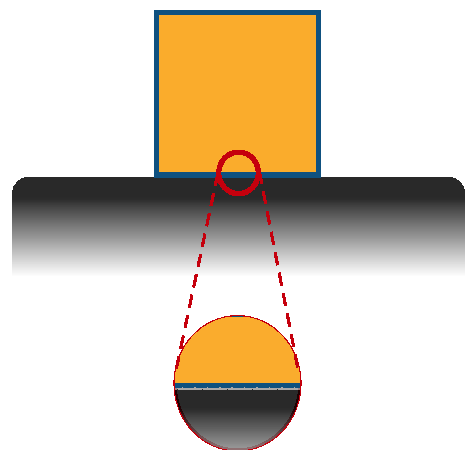
\includegraphics[scale=0.5]{P1} \end{center}

\subsection{Сила тертя спокою}
Нехай на поверхні лежить блок. До нього прикладено дві сили: сила тяжіння $m\vec{g}$ та сила реакції опори $\vec{N}$. Другий закон Ньютона справджується. Дві сили урівноважують одна одну і маємо нульове прискорення. 
\begin{center} 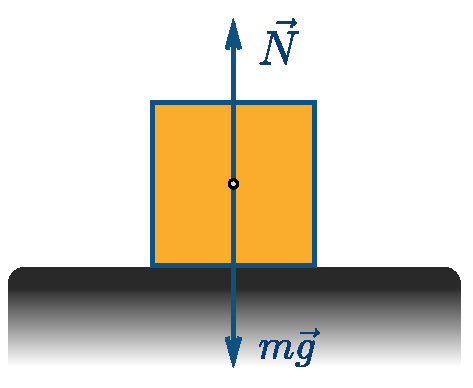
\includegraphics[scale=0.5]{P2} \end{center}

Тепер починаємо прикладати невелику силу до тіла, а воно все одно поки не рухається. Зрозуміло, що для того, щоб другий занкон Ньютона продовжував виконуватися, повинна з'явитися сила, яка урівноважує силу, яку ми приклали до тіла. Це сила тертя $\vec{F}_T$.\\

\textit{Ми з вами домовилися, що для легкості зображення позначатимемо всі сили, прикладені до тіла з рівномірним розподілом маси, використовуючи наближення матеріальної точки. Взагалі то, сила тертя, наприклад, повинна йти вздовж поверхні, а сила реакції опори від самої опопри. Коли буде важливо враховувати форму і точку прикладання сили, ми це обов'язково будемо робити. }\begin{center} 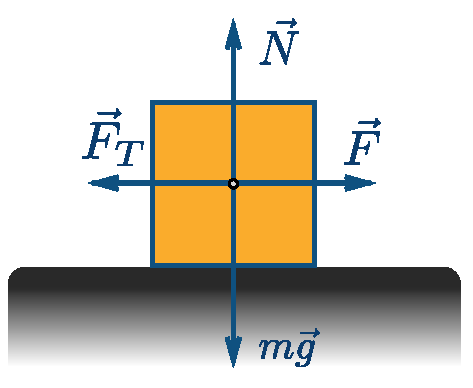
\includegraphics[scale=0.5]{P3} \end{center}
Сила тертя, яка виникає між поверхнею та тілом, коли воно ще нерухоме, називається \textcolor{EdErablue}{\textbf{силою тертя спокою}}.  Для того, щоб прискорення тіла дорівнювало нулю, сила тертя спокою повинна дорівнювати прикладеній силі. $$F_T = F$$\\

Тепер намагаємось все ж таки зрушити тіло, приклавши більшу силу, а воно знову не рухається. Таким чином виходить, що сила тертя спокою знову дорівнює прикладеній силі. \begin{center} 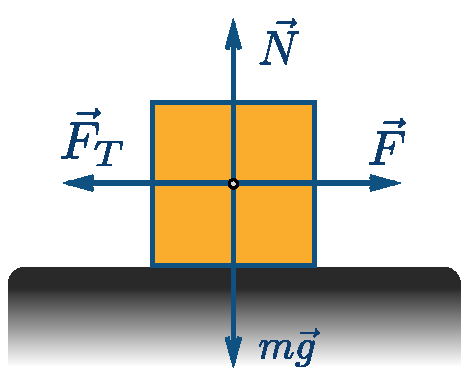
\includegraphics[scale=0.5]{P4} \end{center}
В певний момент нашої прикладеної сили достатньо, щоб зрушити тіло. У цю переломну мить сила тертя спокою набуває свого \textbf{максимального значення} $F^\text{с}_{Tmax}$. Верхній індекс "с" \thinspace означає, що ми розглядаємо силу тертя спокою. \\

Давайте визначемо від чого залежить це максимальне значення.\\

По-перше, воно залежить від того, як сильно взаємодіють між собою поверхня та тіло. Сила, яка відповідає за таку взаємодію – \textcolor{EdErablue}{\textbf{сила реакції опори $N$}}.\\ \newline

По-друге, існує залежність від матеріалів дотичних поверхонь. Коефіцієнт, який характеризує тертя між матеріалами у стані спокоюю називається \textcolor{EdErablue}{\textbf{коефіцієнтом тертя спокою} $\mu_{\text{c}}$ }.\\

\eoz{\textbf{Сила тертя спокою} $F^c_T$ – сила, що виникає при спробі зрушити тіло. \,\,\,Напрямлена вздовж лінії стику поверхонь та в протилежну сторону до напрямку зсуву.\\ \newline
Сила тертя спокою змінюється в межах від нуля (відсутня прикладена сила) до максимального значення $\mu_c N$ (момент початку руху тіла): $$0\le F^c_T\le \mu_c N$$}
\newpage

\subsection{Сила тертя ковзання}
Після того, як ви зрушили тіло, тобто приклали потрібну силу $F = \mu_c N$, тіло починає ковзати по поверхні. Тепер у дію вступає \textcolor{EdErablue}{\textbf{сила тертя ковзання} $F^k_T = \mu_k N$}. \begin{center} 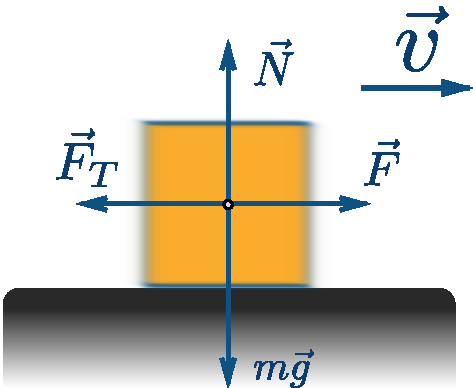
\includegraphics[scale=0.5]{P5} \end{center}
Щоб тіло ковзало з рівномірною швидкістю за другим законом Ньютона $$\boxed{F = F_T = \mu_k N}$$
Сила тертя ковзання на відміну від сили тертя спокою – постійна. Вона не залежить від прикладеної сили. Якщо прикладена сила буде більшою за силу тертя ковзання – тіло буде рухатись з прискоренням, якщо рівною – з постійною швидкістю. \\

\textcolor{red}{\textbf{Більш того!}} Якщо самостійно провести аналіз, не важко пересвідчитися, що зсунути тіло важче, ніж потім штовхати його з рівномірною швидкістю. Максимальна сила тертя спокою (сила, яку требя прикласти, щоб зрушити тіло) більша за силу тертя ковзання. Тому є різниця між коефіцієнтами тертя спокою $\mu_c$ та ковзання $\mu_k$. $$\boxed{\mu_c > \mu_k}$$
\begin{center} 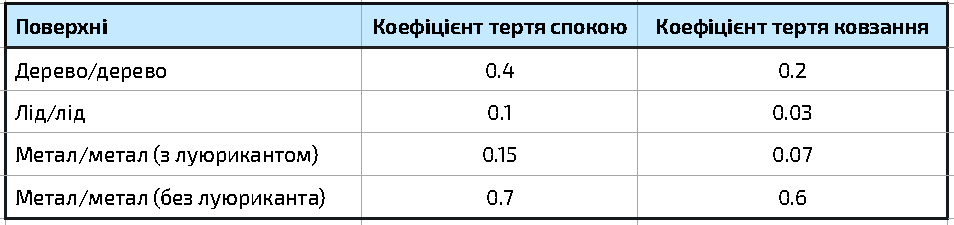
\includegraphics[scale=1]{P6} \end{center}
У \textbf{ЗНО} та шкільній фізиці взагалі часто використовують лише коефіцієнт тертя ковзання. Отже, коли не сказано який саме коефіцієнт дано, то це означає, що мається на увазі коефіцієнт тертя ковзання. \newpage

Давайте побудуємо графік залежності сили тертя від прикладеної сили. \begin{center} 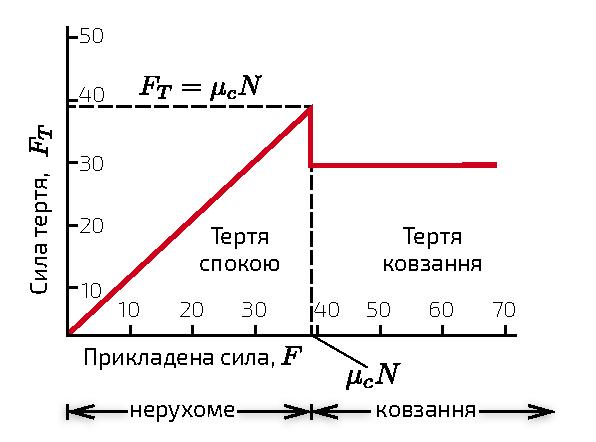
\includegraphics[scale=1]{Vector1} \end{center} \begin{itemize} \item[\textbf{1.}] Поки тіло у спокої, збільшення прикладеної сили $\vec{F}$ викликає пропорційне збільшення сили тертя спокою і при цьому $F_T = F $ \item[\textbf{2.}] Коли прикладена сила стає рівною $F = \mu^c N$, тіло зрушується з місця. \item[\textbf{3.}] При русі тіла діє постійна сила тертя ковзання $F_T = \mu^k N < \mu^c N$. \end{itemize}
\textit{Шкала графіка зображена для випадку з коефіцієнтом тертя спокою $\mu_c = 0.4$, коефіцієнтом тертя ковзання $\mu_k = 0.3$, масою тіла $10$ кг на горизонтальній площині. }
\newpage
\begin{eeprob}{1}{ШТОВХАТИ ЧИ ТЯГТИ?}{Уявіть ситуацію: вам потрібно покатати на санках маленького Петра (ім'я не впливає на розв'язок задачі). В якому випадку вам потрібно прикладати меншу силу, щоб з постійною швидкістю везти санки? \begin{center}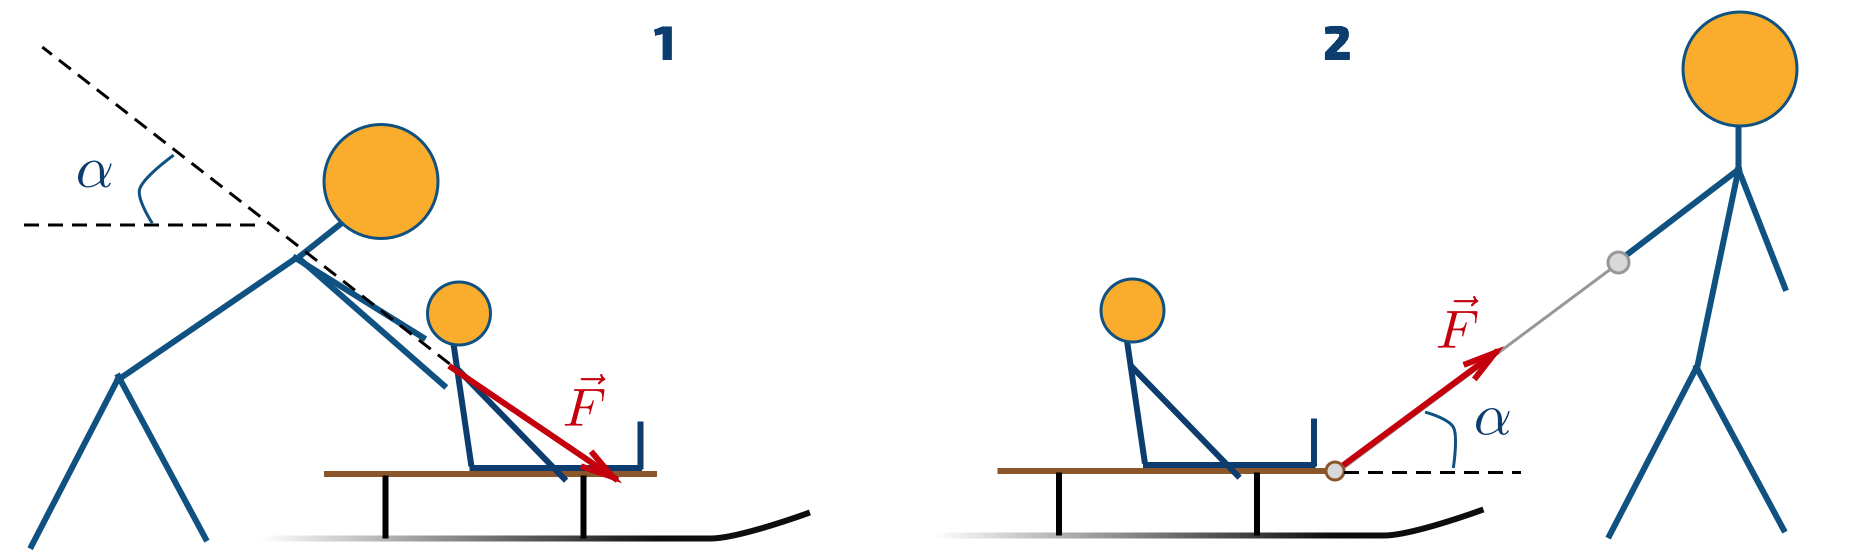
\includegraphics[scale=0.4]{P7}\end{center} Давайте зобразимо всі діючі сили на санки у двох випадках. \begin{center}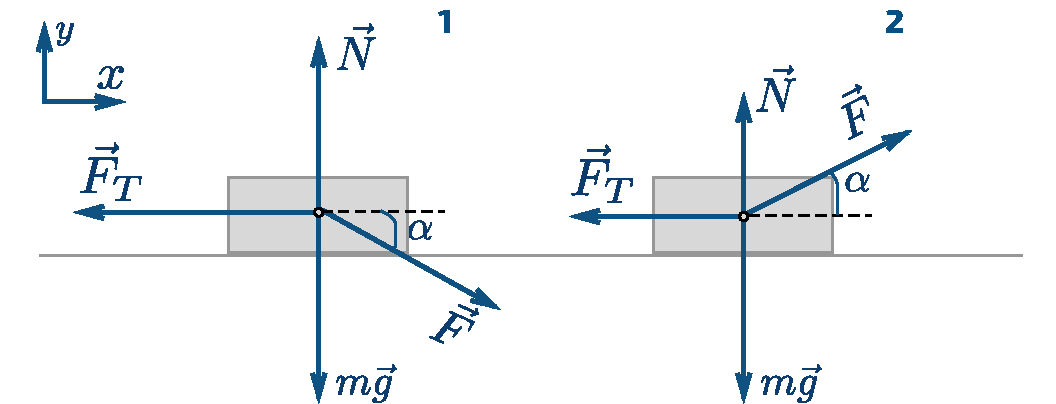
\includegraphics[scale=0.4]{P8}\end{center} \begin{itemize} \item[\textbf{1.}] Другий закон Ньютона: $\vec{F} + \vec{F}_T + \vec{N} + m\vec{g} = 0$. 

Проекція на вісь $y$: $-mg + N - F\sin \alpha = 0\,\,\Rightarrow\,\, \boxed{N = mg +  F\sin \alpha}$


Проекція на вісь $x$: $F\cos \alpha - F_T = 0\,\,\Rightarrow\,\,F = \dfrac{F_T}{\cos\alpha}$ – прикладена сила

Сила тертя ковзання: $F_T = \mu N$. Підставимо отриману силу $N$ $$F_T = \mu N = \mu (mg + F\sin\alpha)\,\,\Rightarrow\,\,\boxed{F = \dfrac{\mu (mg + F\sin\alpha)}{\cos \alpha}}$$ 

\item[\textbf{2.}] Другий закон Ньютона: $\vec{F} + \vec{F}_T + \vec{N} + m\vec{g} = 0$. 

Проекція на вісь $y$: $-mg + N + F\sin \alpha = 0\,\,\Rightarrow\,\, \boxed{N = mg -  F\sin \alpha}$


Проекція на вісь $x$: $F\cos \alpha - F_T = 0\,\,\Rightarrow\,\,F = \dfrac{F_T}{\cos\alpha}$ – прикладена сила

Сила тертя ковзання: $F_T = \mu N$. Підставимо отриману силу $N$ $$F_T = \mu N = \mu (mg + F\sin\alpha)\,\,\Rightarrow\,\,\boxed{F = \dfrac{\mu (mg - F\sin\alpha)}{\cos \alpha}}$$
\end{itemize} Як бачите у другому випадку вертикальна складова прикладеної сили напрямлена в протилежну сторону до сили тяжіння, тим самим зменшуючи силу реакції опори $N$. В свою чергу сила тертя, що пропорційна $N$, також менше. \newline

\textbf{Відповідь: тягти.}}\end{eeprob}
\newpage
\subsubsection{Тіло на вертикальній стінці}
Розповсюджений приклад, в якому головним чином використовується зв'язок сили реакції опори та сили тертя, тіло на вертикальній стінці. Для того, щоб тіло трималося на ній, повинна бути прикладена \textbf{перпендикулярна до її поверхні складова сили}. 
\begin{center}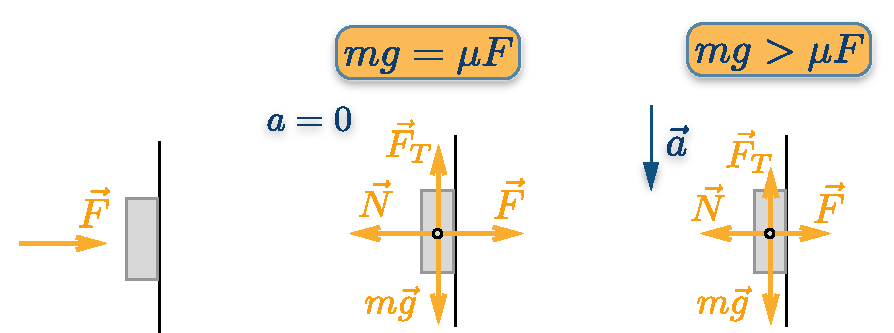
\includegraphics[scale=1]{P9}\end{center}
Наприклад, якщо сказано, що маса тіла 1 кг, коефіцієнт тертя між тілом та стінкою $\mu = 0.2$, а визначити необхідно з якою силою потрібно подіяти на тіло в перпендикулярному до стінки напрямі, щоб воно залишалося нерухомим. До речі, в цьому прикладі в умові дано лише один коефіцієнт тертя. Це до того, що в шкільних задачах часто не відрізняють коефіцієнт тертя спокою та ковзання. \\

\hspace{-0.65cm}\textbf{Щоб тіло було нерухомим}, за другим законом Ньютона: $$mg = F_T = \mu N$$ Сила реакції опори дорівнює перпендикулярній до поверхні стінки складовій силі. В даному випадку $N = F$.\\ 

Cила, яку потрібно прикласти, щоб тіло залишалося нерухомим:
$$mg = \mu F\,\,\Rightarrow\,\, F = \dfrac{mg}{\mu} = \dfrac{1\cdot 9.8}{0.2} = 49 \thinspace (H)$$ 
\newpage

\subsection{Тіло на похилій площині}
Багато задач стосується тіл, які знаходяться на похилій площині. 
\begin{center}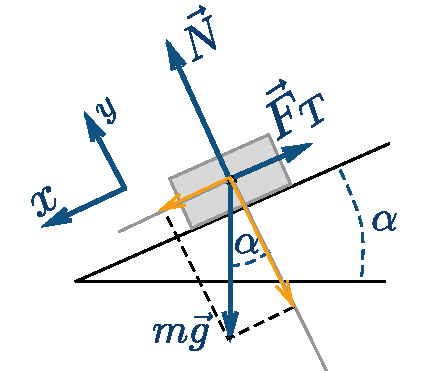
\includegraphics[scale=0.8]{P10}\end{center}
Будемо розбиратися з цим типом завдань на конкретних експериментах. \\

\begin{center}\textcolor{EdErablue}{\textbf{Експеримент 1:}} \textbf{як визначити коефіцієнт тертя? } \end{center}
Нехай у нас є тіло та похила площина, кут нахилу якої ми можемо змінювати і метрична лінійка.\\

Повільно збільшуючи кут нахилу площини, спостерігаємо за поведінкою тіла. При досягненні певного кута $\alpha$ тіло зрушиться і почне "сповзати" \thinspace вниз. Давайте розберемо цей переломний момент. Фактично момент початку руху означає, що сила тертя вже дорівнює своєму максимальному значенню $\mu N$. Вісь $x$ в цьому випадку дуже зручно розмістити вздовж поверхні, тоді вісь $y$ – перпендикулярна і напрямлена вздовж напрямку сили реакції опори $\vec{N}$. Вважаємо, що у момент початку руху прискорення ще дорівнює нулю. \\

Другий закон Ньютона: $$m\vec{g} + \vec{N} + \vec{F}_T = 0$$

Вісь $x$: $$mg\sin \alpha - F_T = 0\,\,\Rightarrow\,\,F_T = mg\sin \alpha$$

Вісь $y$: $$ -mg\cos \alpha + N = 0\,\,\Rightarrow\,\,N = mg\cos\alpha$$ 

Нагадую, що в момент зрушення тіла $F_T = \mu N$. Підставимо у вираз для сили тертя: $$\mu N = mg \sin \alpha\,\,\Rightarrow\,\,\mu mg \cos \alpha = mg \sin \alpha\,\,\Rightarrow\,\,\boxed{\mu = \dfrac{\sin \alpha}{\cos \alpha} = tg \alpha}$$ 

Ми отримали вираз для коефіцієнта тертя. Тепер використавши лінійку, яку ми мали, можемо використати те, що тангенс дорівнює протилеглому катету поділеному на прилеглий.\\

\textcolor{red}{\textbf{Важливо !}} Коефіцієнт тертя не залежить від маси тіла та площі стику поверхонь. \begin{center}\textcolor{EdErablue}{\textbf{Коефіцієнт тертя залежить лише від матеріалів стичних поверхонь. }} \end{center}\newpage
\begin{center}\textcolor{EdErablue}{\textbf{Експеримент 2:}} \textbf{в який бік рухається система? } \end{center}
Маємо два тіла з масами $m_1$ та $m_2$. Визначити умови для трьох станів системи: 1) стан спокою системи; 2) прискорення другого тіла напрямлене вгору; 3) прискорення другого тіла напрямлене вниз.
\begin{center}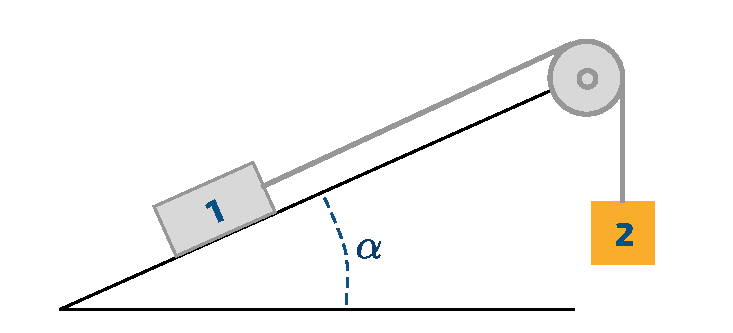
\includegraphics[scale=0.7]{P11} \end{center}

\begin{itemize}
\item \textbf{Момент перед початком руху другого тіла вниз}\\
У цей момент сила тертя, що діє на перше тіло напрямлена вниз по похилій площині. Прискорення у цей момент ще дорівнює нулю. Сила тертя дорівнює максимальній силі тертя спокою $\mu N$.\\
\begin{center}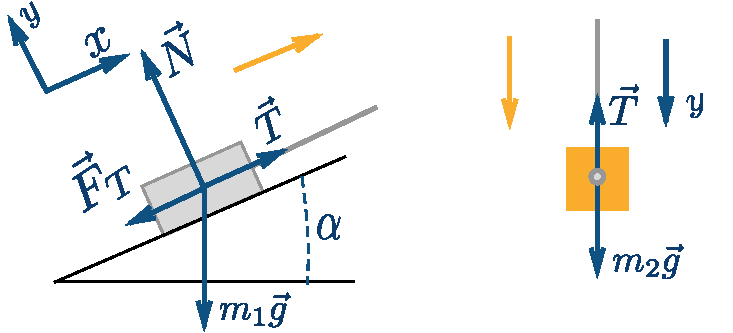
\includegraphics[scale=0.5]{P12} \end{center}
Проекція на вісь $x$ для першого тіла: $$T - F_T - m_1g\sin \alpha = 0\,\,\Rightarrow\,\,T = m_1g\sin \alpha + F_T$$
Проекція на вісь $y$ для другого тіла: $T = m_2g$\\
Сила натягу нитки для першого і для другого тіла – однакова, адже маємо один нерозтяжний трос, що сполучає ці тіла. \\

\textcolor{EdErablue}{\textbf{Умова руху другого тіла вниз: $$\boxed{m_2g \geq m_1g\sin \alpha + F_T}$$}}
\textit{Силу тертя у момент початку руху дорівнює $F_T = \mu N$. $N$ можна визначити за допомогою розгляду проекцій сил, що прикладені до першого тіла,  на вісь $y$. }\newpage
\item \textbf{Момент перед початком руху другого тіла вгору}\\
Тут відмінність у тому, що сила тертя для першого тіла тепер напрямлена в іншу сторону. Тобто співпадає по напрямку з силою натягу нитки. Далі проводимо аналогічні до першого випадку розрахунки. \\
\begin{center}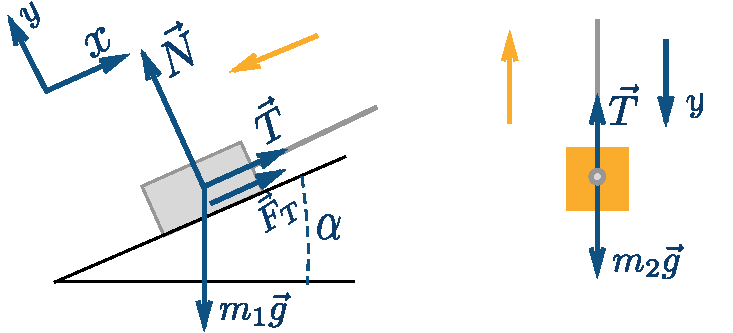
\includegraphics[scale=0.5]{P13} \end{center}
Проекція на вісь $x$ для першого тіла: $$T + F_T - m_1g\sin \alpha = 0\,\,\Rightarrow\,\,T = m_1g\sin \alpha - F_T$$
Проекція на вісь $y$ для другого тіла: $T = m_2g$\\
Знову-таки сила натягу однакова для першого і другого тіла. \\

\textcolor{EdErablue}{\textbf{Умова руху другого тіла вниз: $$\boxed{m_2g \le m_1g\sin \alpha - F_T}$$}}
\end{itemize}

\end{document}

